\documentclass[a4paper, 9pt]{extarticle}
% (1) Encoding, Fonts, and Layout
\usepackage[T1]{fontenc}
\usepackage{lmodern}
\usepackage[margin=1in]{geometry}


% (2) Common Packages
\usepackage{amsmath, amssymb, amsthm}
\usepackage{xcolor}
\usepackage{caption}
\usepackage{tikz}
\usepackage{pgfplots}
\pgfplotsset{compat=newest}
\usepackage{etoolbox}
\usepackage{tikz-3dplot}
\tdplotsetmaincoords{75}{120}
\usepackage[inline]{enumitem}
\usepackage{bookmark}
\usepackage{mathtools}
\usepackage{subcaption} % For subfigures
\usepackage[normalem]{ulem} % For better underline commands

% Micro-typography
\usepackage{microtype}

% Patching pgfplots warning
\makeatletter
\patchcmd{\pgfplots@applistXXpushback@smallbuf}{\pgfplots@error}{\pgfplots@warning}{}{}
\makeatother

% (3) tcolorbox and Theorem Libraries
\usepackage{tcolorbox}
\tcbuselibrary{theorems}

% (4) Define Colors
\definecolor{custom_green}{HTML}{a3be8c}
\definecolor{custom_red}{HTML}{dc322f}
\definecolor{custom_blue}{HTML}{268bd2}
\definecolor{custom_purple}{HTML}{b48ead}

\definecolor{base}{HTML}{eceff4}
\definecolor{gray1}{HTML}{e5e9f0}
\definecolor{gray2}{HTML}{d8dee9}
\definecolor{gray3}{HTML}{2e3440}
\pagecolor{base}

% (5) Custom tcolorbox Environments
\newtcolorbox{definitionbox}[1][]{
    title=\textbf{Definition} {#1},
    fonttitle=\bfseries\boldmath,
    arc=0mm,
    bottomtitle=0.5mm,
    boxrule=0mm,
    colbacktitle=gray2,
    colback=gray1,
    coltitle=gray3,
    coltext=gray3,
    left=2.5mm,
    leftrule=1mm,
    rightrule=1mm,
    right=3.5mm,
    toptitle=0.75mm,
    colframe=custom_red,
}

\newtcolorbox{proofbox}{
    title=\textbf{Proof},
    fonttitle=\bfseries\boldmath,
    arc=0mm,
    bottomtitle=0.5mm,
    boxrule=0mm,
    colbacktitle=gray2,
    colback=gray1,
    coltitle=gray3,
    left=2.5mm,
    leftrule=1mm,
    rightrule=1mm,
    right=3.5mm,
    toptitle=0.75mm,
    colframe=custom_blue,
    coltext=gray3,
}

\newtcolorbox{theorembox}[1][]{
    title=\textbf{Theorem} {#1},
    fonttitle=\bfseries\boldmath,
    arc=0mm,
    bottomtitle=0.5mm,
    boxrule=0mm,
    colbacktitle=gray2,
    colback=gray1,
    coltitle=gray3,
    left=2.5mm,
    leftrule=1mm,
    rightrule=1mm,
    right=3.5mm,
    toptitle=0.75mm,
    colframe=custom_green,
    coltext=gray3
}

\newtcolorbox{notebox}{
    title=\textbf{Note},
    fonttitle=\bfseries\boldmath,
    arc=0mm,
    bottomtitle=0.5mm,
    boxrule=0mm,
    colbacktitle=gray2,
    coltitle=gray3,
    left=2.5mm,
    leftrule=1mm,
    rightrule=1mm,
    right=3.5mm,
    toptitle=0.75mm,
    colframe=custom_blue,
    coltext=gray3
}

\newtcolorbox{examplebox}[1][]{
    title=\textbf{Example} {#1},
    fonttitle=\bfseries\boldmath,
    arc=0mm,
    bottomtitle=0.5mm,
    boxrule=0mm,
    colbacktitle=gray2,
    colback=gray1,
    coltitle=gray3,
    left=2.5mm,
    leftrule=1mm,
    rightrule=1mm,
    right=3.5mm,
    toptitle=0.75mm,
    colframe=gray3,
    fontupper=\footnotesize,
    coltext=gray3
}

% (6) Theorem Environments
\theoremstyle{definition}
\newtheorem{definition}{Definition}[section]
\newtheorem{example}[definition]{Example}

\theoremstyle{plain}
\newtheorem{theorem}[definition]{Theorem}

% (7) Hyperlinks
\usepackage{hyperref}
\hypersetup{
    colorlinks=true,    % Use colored text for links
    linkcolor=custom_red,      % Set link text color to red
    pdfborder={0 0 0}   % Remove the default box around links
}

% macros.tex
\newcommand{\intinf}{\int_0^{\infty}} % Integral from 0 to infinity
\newcommand{\diff}[2]{\frac{d#1}{d#2}} % Derivative


\title{
\textbf{MA283: Linear Algebra} \\ 
}

\usepackage{geometry}
 \geometry{
 a4paper,
 bottom=22mm,
 }

\author{
  70\% Exam\\
30\% Continuous Assessment (Homework) \\
10\% Optional Project (Bonus)\\ [2ex]
Robert Davidson
}     
\date{}       % Optional: Add date if desired

\begin{document}

\maketitle
\pagebreak

\tableofcontents
\pagebreak
\section{Review of Matrix Algebra}
\subsection*{Matrix Addition}
If a matrix has $m$ rows and $n$ columns, we say it is $m \times n$.\textbf{Two matrices can only be added if they have the same size.}. In this case, we just add the entries in each position. \\[2ex]
The $m \times n$ \textbf{zero} matrix is a matrix with all entries equal to $0$. It is the \textbf{Identity element} for matrix addition (adding it to any matrix does not change the matrix)
\subsection*{Matrix Multiplication by a Scalar}
This simply means multiplying each entry of the matrix by the scalar. For example:
$$
  \alpha \begin{bmatrix}
    1 & 2 \\
    3 & 4 \\
  \end{bmatrix}
  =
  \begin{bmatrix}
    \alpha  & 2\alpha \\
    3\alpha & 4\alpha \\
  \end{bmatrix}
$$

\textbf{Remark}: Now that we have addition and scalar multiplication, we can subtract matrices ($A - B = A + (-1)B$), provided they are the same size.

\subsection*{Vector Space}
With these operations of addition and scalar multiplication, the set of
$m \times n$ matrices is a vector space. A \textbf{vector space} algebraic structure whose elements can be added, subtracted and multiplied by scalars.

\subsection*{Linear Combinations}
\begin{definitionbox}{Linear Combinations}{}
  Suppose $v_1, v_2, \dots, v_k$ are elements that can be added together and multiplied by scalars. \\[2ex]
  A Linear Combination of $v_1, v_2, \dots, v_k$ is an expression of the form:
  $$
    \alpha_1 v_1 + \alpha_2 v_2 + \ldots + \alpha_k v_k
  $$
  where $a_i \in \mathbb{R}$ are scalars, called \textbf{coefficients}.
\end{definitionbox}
\subsection*{Matrix-Vector Multiplication}
\begin{definitionbox}{}{}
  Let $A$ be a $m \times n$ matrix, and $\textbf{v}$ be a column vector with $n$ entries ($n \times 1$ matrix). \\[2ex]
  Then the matrix vector product $Av$ is the column vector, with $m$ entries, obtained by taking the linear combination of the columns of $A$ with the entries of $\textbf{v}$ as coefficients.
  \\ \rule{\textwidth}{1px} \\
  $$
    \begin{bmatrix}
      -1 & 2 & 4 \\
      0  & 1 & 3
    \end{bmatrix}
    \begin{bmatrix}
      7 \\
      6 \\
      9
    \end{bmatrix}
    =
    7 \begin{bmatrix}
      -1 \\
      0
    \end{bmatrix}
    + 6 \begin{bmatrix}
      2 \\
      1
    \end{bmatrix}
    + 9 \begin{bmatrix}
      4 \\
      3
    \end{bmatrix}
    =
    \begin{bmatrix}
      41 \\
      33
    \end{bmatrix}.
  $$
  \rule{\textwidth}{1px} \\[2ex]
  \textbf{Remark:} $Av$, if defined, has the same number of rows as $A$ and the same number of columns as $\textbf{v}$.
\end{definitionbox}

\subsection*{Matrix-Matrix Multiplication}
\begin{definitionbox}{}{}
  Let $A$ and $B$ be matrices of size $m \times p$ and $p \times n$, respectively.Write $v_1, \ldots v_n$ for the columns of $B$. Then the product $AB$ is the $m \times n$ matrices whose columns are $Av_1 , \ldots, Av_n$.
  \\ \rule{\textwidth}{1px} \\
  The entry at row $i$ and column $j$ of the matrix $A$ is given by $A_{ij}$. The entry in the $i,j$ position of the product $AB$ is the $i$th entry of the vector $Av_j$, where the vector $v_j$ is the $j$th column of $B$. In other words, the entry in the $i,j$ position of the product $AB$ is given by:
  $$
    (AB)_{ij} = A_{i1}B_{1j} + A_{i2}B_{2j} + \ldots + A_{ip}B_{pj} = \sum_{k=1}^p A_{ik}B_{kj}
  $$
\end{definitionbox}
\begin{definitionbox}{}{}
  If $A$ is $m \times p$ with rows $u_1, \ldots, u_m$ and $B$ is $p \times n$ with columns $v_1, \ldots, v_n$, then the product $AB$ is:
  $$AB =
    \begin{bmatrix}
      u_1 \cdot v_1 & u_1 \cdot v_2 & \ldots & u_1 \cdot v_n \\
      u_2 \cdot v_1 & u_2 \cdot v_2 & \ldots & u_2 \cdot v_n \\
      \vdots        & \vdots        & \ddots & \vdots        \\
      u_m \cdot v_1 & u_m \cdot v_2 & \ldots & u_m \cdot v_n
    \end{bmatrix}
  $$
  \rule {\textwidth}{1px} \\[2ex]
  \textbf{Example}:
  $$
    A =
    \begin{bmatrix}
      1 & 2 & 3 \\
      4 & 5 & 6
    \end{bmatrix}
    \quad
    B =
    \begin{bmatrix}
      7  & 8  \\
      9  & 10 \\
      11 & 12
    \end{bmatrix}
    \quad
    AB =
    \begin{bmatrix}
      1 \cdot 7 + 2 \cdot 9 + 3 \cdot 11 & 1 \cdot 8 + 2 \cdot 10 + 3 \cdot 12 \\
      4 \cdot 7 + 5 \cdot 9 + 6 \cdot 11 & 4 \cdot 8 + 5 \cdot 10 + 6 \cdot 12
    \end{bmatrix}
    =
    \begin{bmatrix}
      58  & 64  \\
      139 & 154
    \end{bmatrix}
  $$
\end{definitionbox}
For matrices $A$ and $B$, the products $AB$ and $BA$ are generally not
equal, even if they are both defined and even if both have the same
size.
\subsection*{Linear Transformations}
\begin{definitionbox}{}{}
  Let $m$ and $n$ be positive integers. \\[2ex]
  A \textbf{linear transformation} $T$ from $\mathbb{R}^n$ to $\mathbb{R}^m$ is a function $T:\mathbb{R}^n \to \mathbb{R}^m$ that satisfies:
  \begin{itemize}
    \item $T(\textbf{u} + \textbf{v}) = T(\textbf{u}) + T(\textbf{v})$ for all $\textbf{u}, \textbf{v} \in \mathbb{R}^n$
    \item $T(\lambda\textbf{u}) = \lambda T(\textbf{u})$ for all $\textbf{u} \in \mathbb{R}^n$ and $\lambda \in \mathbb{R}$
  \end{itemize}
\end{definitionbox}
\subsection*{Matrix of a Linear Transformation}
Suppose $T:\mathbb{R}^3 \to \mathbb{R}^2$ is the linear transformation:
$$
  T\begin{bmatrix}
    1 \\
    0 \\
    0 \\
  \end{bmatrix}
  = \begin{bmatrix}
    2 \\
    3 \\
  \end{bmatrix}
  \quad
  T\begin{bmatrix}
    0 \\
    1 \\
    0 \\
  \end{bmatrix}
  = \begin{bmatrix}
    1 \\
    4 \\
  \end{bmatrix}
  \quad
  T\begin{bmatrix}
    0 \\
    0 \\
    1 \\
  \end{bmatrix}
  = \begin{bmatrix}
    -6 \\
    7  \\
  \end{bmatrix}
$$
Then for the vector in $\mathbb{R}^3$ with entries $a,b,c$:
$$
  T\begin{bmatrix}
    a \\
    b \\
    c \\
  \end{bmatrix}
  = aT\begin{bmatrix}
    1 \\
    0 \\
    0 \\
  \end{bmatrix}
  + bT\begin{bmatrix}
    0 \\
    1 \\
    0 \\
  \end{bmatrix}
  + cT\begin{bmatrix}
    0 \\
    0 \\
    1 \\
  \end{bmatrix}
  = \begin{bmatrix}
    2  & 1 & -6 \\
    -3 & 4 & 7
  \end{bmatrix}
  \begin{bmatrix}
    a \\
    b \\
    c
  \end{bmatrix}
$$
Where the $2\times 3$ matrix $M_T$ is called the \textbf{standard matrix} of A.
A linear transformation $T: \mathbb{R}^n \rightarrow \mathbb{R}^m$ can be completely represented by an $m \times n$ matrix $M_T$. \\[2ex]
\textbf{Understanding the Matrix Representation}
\begin{itemize}
  \item The columns of matrix $M_T$ are the images of the standard basis vectors $e_1, e_2, \ldots, e_n$ under $T$.
  \item For any vector $v \in \mathbb{R}^n$, we calculate $T(v)$ by multiplying: $M_T \cdot v$.
  \item Therefore, matrix-vector multiplication is simply evaluating a linear transformation.
\end{itemize}
\textbf{Correspondence:} Any $m \times n$ matrix $A$ defines a linear transformation $T_A: \mathbb{R}^n \rightarrow \mathbb{R}^m$ by: $T_A(v) = Av$. Linear transformations include rotations, reflections and scaling \\[2ex]
\textbf{Efficiency of Representation:} A remarkable property of linear transformations is their information efficiency:
\begin{itemize}
  \item To completely define $T: \mathbb{R}^n \rightarrow \mathbb{R}^m$, we need only $mn$ values.
  \item These values are the coordinates of the $n$ transformed basis vectors in $\mathbb{R}^m$.
  \item This differs fundamentally from general continuous functions $f: \mathbb{R} \rightarrow \mathbb{R}$, which cannot be fully determined by their values at finitely many points.
\end{itemize}
\pagebreak
\subsection*{Matrix multiplication is composition}
Suppose that $T:\mathbb{R}^n \to \mathbb{R}^p$ and $S:\mathbb{R}^p \to \mathbb{R}^m$ are linear transformations. Then the composition $S \circ T: \mathbb{R}^n \to \mathbb{R}^m$ is also a linear transformation from $\mathbb{R}^n$ to $\mathbb{R}^m$ defined for $\mathbf{v} \in \mathbb{R}^n$ by:
$$
  S \circ T(\mathbf{v}) = S(T(\mathbf{v}))
$$
To see how that the $m \times n$ matrix $M_{S\circ T}$ depends on the matrix $M_S (m \times p)$ and $M_T (p \times n)$ we look at the definition of $M_{S\circ T}$:
\begin{itemize}
  \item The first column has coordinates $S\circ T(e_1) = S(T(e_1))$
  \item $T(e_1)$ is first column of $M_T$
  \item Then $S(T(e_1))$ is the matrix-vector product $M_S \cdot M_T(e_1)$
  \item Same for all other columns $\Longrightarrow$ $M_{S\circ T} = M_S \cdot M_T$
\end{itemize}
Thus, we conclude $\textbf{matrix multiplication is composition of linear transformations}$.
\pagebreak
\section{Systems of linear equations}
\subsection{Linear equations and Solution Sets}
A linear equation in the variables $x$ and
$y$ is an equation of the form
\begin{equation*}
  2x + y = 3
\end{equation*}
If we replace $x$ and $y$ with some numbers, the statement \textbf{becomes true or false}.

\begin{definitionbox}{Solution to a linear equation}{}
  A pair, $(x_0, y_0) \in \mathbb{R}$, is a solution to an linear equation if setting $x = x_0$ and $y = y_0$ \textbf{makes the equation true.}
\end{definitionbox}

\begin{definitionbox}{Solution set}{}
  The \textbf{solution set} is the set of all solutions to a linear equation.
  $$a_1X_1 + a_2X_2 + \ldots + a_nX_n = b \quad \text{where} \; a_i, b \in \mathbb{R}$$
  is an \textbf{affine hyperplane} in $\mathbb{R}^n$; geometrically resembles a copy of $\mathbb{R}^{n-1}$ inside $\mathbb{R}^n$.
\end{definitionbox}
\subsubsection{Interpreting Linear Systems as Matrix Equations}
$$
  \begin{array}{ccccccc}
    x  & + & 2y & - & z  & = & 5 \\
    3x & + & y  & - & 2z & = & 9 \\
    -x & + & 4y & + & 2z & = & 0
  \end{array}
  \quad \Rightarrow \quad
  \begin{bmatrix}
    1  & 2 & -1 \\
    3  & 1 & -2 \\
    -1 & 4 & 2
  \end{bmatrix}
  \begin{bmatrix}
    x \\
    y \\
    z
  \end{bmatrix}
  =
  \begin{bmatrix}
    5 \\
    9 \\
    0
  \end{bmatrix}
$$
\subsection{Elementary Row Operations}
To solve a system of linear equations we associate an \textbf{augmented matrix} to the system of equations. For example:
$$
  \begin{array}
    {ccccccc}x & + & 2y & - & z  & = & 5 \\
    3x         & + & y  & - & 2z & = & 9 \\
    -x         & + & 4y & + & 2z & = & 0
  \end{array}
  \quad \Rightarrow \quad
  \begin{bmatrix}
    1  & 2 & -1 & | & 5 \\
    3  & 1 & -2 & | & 9 \\
    -1 & 4 & 2  & | & 0
  \end{bmatrix}
$$
To solve, we can perform the following \textbf{Elementary Row Operations (EROs)}:
\begin{enumerate}
  \item Multiply a row by a non-zero constant.
  \item Add a multiple of one row to another row.
  \item Swap two rows.
\end{enumerate}
The goal of these operations is to transform the augmented matrix into \textbf{row echelon form} (REF) or \textbf{reduced row echelon form} (RREF).

\subsubsection{REF and Strategy}
\begin{minipage}{0.8\textwidth}
  We say a matrix is in \textbf{row echelon form} (REF) if:
  \begin{itemize}
    \item The first non zero entry in each row is a 1 (called the \textbf{leading 1}).
    \item If a column has a leading 1, then all entries below it are 0.
    \item The leading 1 in each row is to the right of the leading 1 in the previous row.
    \item All rows of 0s are at the bottom of the matrix.
  \end{itemize}
\end{minipage}
\begin{minipage}{0.2\textwidth}
  \begin{center}
    $$
      \begin{bmatrix}
        1 & 2 & -1 & | & 3  \\
        0 & 1 & 2  & | & -1 \\
        0 & 0 & 1  & | & -1
      \end{bmatrix}
    $$
    \emph{Example of REF}
  \end{center}


\end{minipage} \\[2ex]
We have produced a new system of equations. This is easily solved by back substitution.

\begin{conceptbox}{Stategy for Obtaining REF}{}
  \begin{itemize}
    \item Get a 1 as the top left entry
    \item Use this 1 to clear the entries below it
    \item Move to the next column and repeat
    \item Continue until all leading 1s are in place
    \item Use back substitution to solve the system
  \end{itemize}
\end{conceptbox}
\subsubsection{Row Reduced Echelon Form}
\begin{minipage}{0.8\textwidth}
  A matrix is in \textbf{reduced row echelon form} (RREF) if:
  \begin{itemize}
    \item It is in REF
    \item The leading 1 in each row is the only non-zero entry in its column.
  \end{itemize}
\end{minipage}
\begin{minipage}{0.2\textwidth}
  \begin{center}
    $$
      \begin{bmatrix}
        1 & 0 & 0 & | & 2  \\
        0 & 1 & 0 & | & -1 \\
        0 & 0 & 1 & | & -1
      \end{bmatrix}
    $$
    \emph{Example of RREF}
  \end{center}
\end{minipage}

\subsection{Leading variables and free variables}
We'll start by an example:
$$
  \begin{array}{ccccccccc}
    x_1  & - & x_2  & - & x_3  & + & 2x_4 & = & 0 \\
    2x_1 & + & x_2  & - & x_3  & + & 2x_4 & = & 8 \\
    x_1  & - & 3x_2 & + & 2x_3 & + & 7x_4 & = & 2
  \end{array}
  \quad \Rightarrow \quad
  \begin{bmatrix}
    1 & -1 & -1 & 2 & | & 0 \\
    2 & 1  & -1 & 2 & | & 8 \\
    1 & -3 & 2  & 7 & | & 2
  \end{bmatrix}
$$
Solving this system of equations, we get:
$$
  \text{RREF:}\quad
  \begin{bmatrix}
    1 & 0 & 0 & 2  & | & 4 \\
    0 & 1 & 0 & -1 & | & 2 \\
    0 & 0 & 0 & 1  & | & 2
  \end{bmatrix}
  \quad \Rightarrow \quad
  \begin{array}{ccccc}
    x_1 & + & 2x_4 & = & 4 \quad \\
    x_2 & - & x_4  & = & 2 \quad \\
    x_3 & + & x_4  & = & 2 \quad
  \end{array}
  \quad \Rightarrow \quad
  \begin{array}{ccc}
    x_1 & = & 4 - 2x_4 \\
    x_2 & = & 2 + x_4  \\
    x_3 & = & 2 - x_4
  \end{array}
$$
This RREF tells us how the \textbf{leading variables} ($x_1, x_2, x_3$) depend on the \textbf{free variable} ($x_4$). The free variable can take any value in $\mathbb{R}$. We write the solution set as:
$$x_1 = 4 - 2t, \quad x_2 = 2 + t, \quad x_3 = 2 - t, \quad x_4 = t \quad \text{where} \; t \in \mathbb{R}$$
$$(x_1, x_2, x_3, x_4) = (4-2t, 2+t, 2-t, t); \quad t \in \mathbb{R}$$
\begin{definitionbox}{Leading and Free Variables}{}
  \begin{itemize}
    \item  \textbf{Leading variable} : A variable whose columns in the RREF contain a leading 1
    \item \textbf{Free variable} : A variable whose columns in the RREF do not contain a leading 1
  \end{itemize}
\end{definitionbox}

\subsection{Consistent and Inconsistent Systems}
Consider the following system of equations:
$$
  \begin{array}{ccccccc}
    3x & + & 2y & - & 5z & = & 4 \\
    x  & + & y  & - & 2z & = & 1 \\
    5x & + & 3y & - & 8z & = & 6
  \end{array}
  \quad \Rightarrow \quad
  \begin{bmatrix}
    3 & 2 & -5 & | & 4 \\
    1 & 1 & -2 & | & 1 \\
    5 & 3 & -8 & | & 6
  \end{bmatrix}
  \quad \Rightarrow \quad
  \begin{bmatrix}
    1 & 1 & -2 & | & 1 \\
    0 & 1 & -1 & | & 1 \\
    0 & 0 & 0  & | & 1
  \end{bmatrix} \quad \text{(REF)}
$$
We can see the last row of the REF is:
$$
  0x + 0y + 0z = 1
$$
This equation clearly has no solution, and hence the system has no solutions. We say the system is \textbf{inconsistent}. Alternatively, we say the system is \textbf{consistent} if it has at least one solution.
\subsection{Possible Outcomes when solving a system of equations}
\begin{itemize}
  \item The system may be \textbf{inconsistent} (no solutions) - i.e:
        $$ [0 \; 0 \; \dots \; 0 \; | \; a] \quad a \neq 0$$
  \item The system may be \textbf{consistent} which occurs if:
        \begin{itemize}
          \item \textbf{Unique Solutions} each column (aside from the rightmost) contains a single leading 1. - i.e:
                $$
                  \begin{bmatrix}
                    1 & 0 & 0 & | & 4  \\
                    0 & 1 & 0 & | & 3  \\
                    0 & 0 & 1 & | & -2
                  \end{bmatrix}
                $$

          \item \textbf{Infinitely many solutions} at least one variable does not appear as a leading 1 in any row, making it a free variable - i.e:
                $$
                  \begin{bmatrix}
                    1 & 2 & -1 & | & 3  \\
                    0 & 0 & 1  & | & -2 \\
                    0 & 0 & 0  & | & 0
                  \end{bmatrix}
                $$
        \end{itemize}
\end{itemize}

\subsection{Elementary Row Operations as Matrix Transformations}
Elementary row operations may be interpreted as \textbf{matrix multiplication}. To see this, first we introduce the \textbf{Identity matrix:}
\vspace{-2ex}
$$I_3 = \begin{bmatrix}
    1 & 0 & 0 \\
    0 & 1 & 0 \\
    0 & 0 & 1
  \end{bmatrix}$$
The $I_m$ Identity matrix is an $m \times m$ matrix with 1s on the diagonal and 0s elsewhere. We also introduce the $E_{i,j}$ matrix which has $1$ in the $(i,j)$ position and $0$s elsewhere. For example:
$$
  E_{1,2} = \begin{bmatrix}
    0 & 1 & 0 \\
    0 & 0 & 0 \\
    0 & 0 & 0
  \end{bmatrix}
$$
Then:
\vspace{-2ex}
$$I_3 + 4E_{1,2} = \begin{bmatrix}
    1 & 4 & 0 \\
    0 & 1 & 0 \\
    0 & 0 & 1
  \end{bmatrix}$$
Performing a row operation on $A$ is the same as multiplying $A$ by an appropriate matrix $E$ on the left.
These matrices are called \textbf{elementary matrices}. They are \textbf{always invertible,} and \textbf{their inverses are also elementary matrices}. The statement:
$$
  "\emph{every matrix can be reduced to RREF through EROs}"$$
is equivalent to saying that
\begin{align*}
  "\emph{for every matrix $A$ with $m$ rows, there exists a $m \times m$ matrix $B$} \\
  \emph{which is a product of elementary matrices such that $BA$ is in RREF.}"
\end{align*}
\vspace{-8ex}
\subsubsection{Multiplying a Row by a Non-Zero Scalar}
When multiplying row $i$ of matrix $A$ by a scalar $\alpha \neq 0$, we can use the matrix:
$$I_m + (\alpha - 1)E_{i,i}$$
This works because it modifies only the $(i,i)$ entry of the identity matrix to be $\alpha$ while keeping all other entries unchanged. When multiplied with $A$, it scales row $i$ by $\alpha$ and leaves all other rows intact.\\
\textbf{Example:} If $\alpha = 5$ and $i = 2$, then:
\vspace{-2ex}
$$
  I_3 + 4E_{2,2} = \begin{bmatrix}
    1 & 0 & 0 \\
    0 & 5 & 0 \\
    0 & 0 & 1
  \end{bmatrix}\
  \quad
  A = \begin{bmatrix}
    1 & 2 & 3 \\
    4 & 5 & 6 \\
    7 & 8 & 9
  \end{bmatrix}
  \quad \quad\quad
  (I_3 + 4E_{2,2})A = \begin{bmatrix}
    1  & 2  & 3  \\
    20 & 25 & 30 \\
    7  & 8  & 9
  \end{bmatrix}$$
\vspace{-4ex}
\subsubsection{Switching Two Rows}
To swap rows $i$ and $k$, we use:
$$S = I_m + E_{i,k} + E_{k,i} - E_{i,i} - E_{k,k}$$
This works by:
\begin{itemize}
  \item Removing the 1's at positions $(i,i)$ and $(k,k)$ from the identity matrix
  \item Adding 1's at positions $(i,k)$ and $(k,i)$
\end{itemize}
\vspace{-1ex}
\textbf{Example:} Swapping rows 1 and 3:
\vspace{-2ex}
$$  S = \begin{bmatrix}
    0 & 0 & 1 \\
    0 & 1 & 0 \\
    1 & 0 & 0
  \end{bmatrix}
  \quad
  A = \begin{bmatrix}
    1 & 2 & 3 \\
    4 & 5 & 6 \\
    7 & 8 & 9
  \end{bmatrix}
  \quad \quad\quad
  SA = \begin{bmatrix}
    7 & 8 & 9 \\
    4 & 5 & 6 \\
    1 & 2 & 3
  \end{bmatrix}$$
\vspace{-5ex}
\subsubsection{Adding a Multiple of One Row to Another}
To replace row $k$ with row $k + \alpha \times$ row $i$, use:
$$I_m + \alpha E_{k,i}$$
This adds $\alpha$ times row $i$ to row $k$ while leaving all other rows unchanged because:
\begin{itemize}
  \item For any row $j \neq k$, the corresponding row in this matrix is just the standard basis row
  \item Row $k$ becomes the sum of the standard basis row $k$ plus $\alpha$ times the standard basis row $i$
\end{itemize}
\textbf{Example:} Adding 3 times row 1 to row 2:
\vspace{-1ex}
$$ I_3 + 3E_{2,1} = \begin{bmatrix}
    1 & 0 & 0 \\
    3 & 1 & 0 \\
    0 & 0 & 1
  \end{bmatrix} \quad A = \begin{bmatrix}
    1 & 2 & 3 \\
    4 & 5 & 6 \\
    7 & 8 & 9
  \end{bmatrix}
  \quad\quad\quad
  (I_3 + 3E_{2,1})A = \begin{bmatrix}
    1 & 2  & 3  \\
    7 & 11 & 15 \\
    7 & 8  & 9
  \end{bmatrix}$$

\begin{examplebox}{}{}
  Write the inverse of an elementary matrix and show it is an elementary matrix.
  \\ \rule{\textwidth}{1px} \\
  \textbf{Multiplying a row by a nonzero scalar:}
  \begin{itemize}
    \item \textbf{Operation:} Multiply row $i$ by $\alpha \neq 0$.
    \item \textbf{Elementary Matrix:} $E = I_m + (\alpha - 1)E_{i,i}$
    \item \textbf{Inverse:} To reverse the operation, multiply row $i$ by $1\backslash\alpha$. Hence, the inverse is
          $$
            E^{-1} = I_m + \left(\frac{1}{\alpha} - 1\right)E_{i,i}  =\; I_m + \frac{1-\alpha}{\alpha}\,E_{i,i}.
          $$
  \end{itemize}
  \textbf{Swapping two rows:}
  \begin{itemize}
    \item \textbf{Operation:} Swap rows $i$ and $k$.
    \item \textbf{Elementary Matrix:} $S = I_m - E_{i,i} - E_{k,k} + E_{i,k} + E_{k,i}$
    \item \textbf{Inverse:} Since swapping the same two rows twice returns them to their original positions,
          $$
            S^{-1} = S.
          $$
  \end{itemize}
  \textbf{Adding a multiple of one row to another:}
  \begin{itemize}
    \item \textbf{Operation:} Add $\alpha$ times row $i$ to row $k$.
    \item \textbf{Elementary Matrix:} $E = I_m + \alpha\,E_{k,i}$
    \item \textbf{Inverse:} To undo the operation, subtract $\alpha$ times row $i$ from row $k$. Therefore,
          $$
            E^{-1} = I_m - \alpha\,E_{k,i}.
          $$
  \end{itemize}
\end{examplebox}
\begin{examplebox}{}{}
  Prove that every invertible matrix in $M_n(\mathbb{R})$ is a product of elementary matrices.
  \\ \rule{\textwidth}{1px} \\
  Let $A$  be an invertible matrix in $M_n(\mathbb{R})$. Since $A$ is invertible, we can use Gaussian elimination to transform $A$ into the identity matrix $I_n$. \\[2ex]
  Let $E_1, E_2, \ldots, E_k$ be the elementary matrices corresponding to the row operations used in the elimination process. Then, we have:
  \begin{align*}
    \text{Multiplying a row by a scalar:}           & \quad I_n + (\alpha - 1)E_{i,i}                   \\
    \text{Swapping two rows:}                       & \quad I_n + E_{i,k} + E_{k,i} - E_{i,i} - E_{k,k} \\
    \text{Adding a multiple of one row to another:} & \quad I_n + \alpha\,E_{k,i}
  \end{align*}
  Applying these in sequence to $A$ gives:
  $$E_k \cdots E_2 E_1 A = I_n$$
  Since $E_k \cdots E_2 E_1 = I_n$, we can multiply both sides by $(E_k \cdots E_2 E_1)^{-1}$ on the left to obtain:
  $$A = (E_k \cdots E_2 E_1)^{-1} I_n = (E_k \cdots E_2 E_1)^{-1}$$
  Using the property:
  $$(E_k \cdots E_2 E_1)^{-1} = E_1^{-1} E_2^{-1} \cdots E_k^{-1},$$
  we can express $A$ as a product of elementary matrices:
  $$A = E_1^{-1} E_2^{-1} \cdots E_k^{-1}$$
  Since each $E_i$ is an elementary matrix, its inverse is also an elementary matrix. Therefore, $A$ can be expressed as a product of elementary matrices.
\end{examplebox}
\pagebreak
\subsection{EROs and Inverses}
Elementary Row Operations can be used to find the inverse of a square matrix.  Consider a square matrix $A \in M_n(\mathbb{F})$ (that is, an $n \times n$ matrix over a field $\mathbb{F}$). If $A$ is invertible, let
$$
  A^{-1}
  =
  \begin{bmatrix}
    |            & |            &        & |            \\
    \mathbf{v}_1 & \mathbf{v}_2 & \cdots & \mathbf{v}_n \\
    |            & |            &        & |
  \end{bmatrix}
$$
be its inverse, where each $\mathbf{v}_i$ is the $i$th column of $A^{-1}$. By definition of the matrix inverse, we have
$$
  A \, A^{-1}
  =
  A \begin{bmatrix}
    \mathbf{v}_1 & \mathbf{v}_2 & \cdots & \mathbf{v}_n
  \end{bmatrix}
  =
  \begin{bmatrix}
    A \mathbf{v}_1 & A \mathbf{v}_2 & \cdots & A \mathbf{v}_n
  \end{bmatrix}
  =
  I_n,
$$
the $n \times n$ identity matrix. This implies that
$$
  A \mathbf{v}_i = \mathbf{e}_i, \quad \text{for each } i=1, 2, \ldots, n,
$$
where $\mathbf{e}_i$ is the $i$th column of $I_n$ (which has a 1 in the $i$th row and 0 everywhere else). In other words, each column $\mathbf{v}_i$ of $A^{-1}$ is the unique solution to the linear system
$$
  A \mathbf{v}_i = \mathbf{e}_i.
$$
To find $A^{-1}$ effectively, we form the augmented matrix $[A \mid I_n]$ and apply EROs to trasnform $A$ into $I_n$. When this is achieved, the augmented portion becomes $A^{-1}$. Thus, we have
$$
  \text{RREF}\bigl([\,A \mid I_n\,]\bigr)
  =
  \bigl[\, I_n \mid A^{-1} \bigr].
$$
\begin{examplebox}{}{}
  Find $A^{-1}$ if $A = \begin{bmatrix}
      3 & 4 & -1 \\
      1 & 0 & 3  \\
      2 & 5 & -4
    \end{bmatrix}$.
  \\[2ex] \rule{\textwidth}{1px} \\
  We form a $3 \times 6$ matrix $A' = [A \mid I_3]$:
  $$
    A' = \begin{bmatrix}
      3 & 4 & -1 & | & 1 & 0 & 0 \\
      1 & 0 & 3  & | & 0 & 1 & 0 \\
      2 & 5 & -4 & | & 0 & 0 & 1
    \end{bmatrix}
  $$
  We apply the following EROs to $A'$:
  \begin{itemize}
    \item $R_1 \leftrightarrow R_2$
    \item $R_2 \rightarrow R_2 - 3R_1$
    \item $R_3 \rightarrow R_3 - 2R_1$
    \item $R_3 \rightarrow R_3 + R-2$
    \item $R_3 \leftrightarrow R_2$
    \item $R_3 \rightarrow R_3 - 4R_2$
    \item $R_3 \times (-\frac{1}{10})$
    \item $R_1 \rightarrow R_1 - 3R_3$
  \end{itemize}
  To obtain:
  $$
    \begin{bmatrix}
      1 & 0 & 0 & | & \frac{3}{2}  & -\frac{11}{10} & -\frac{6}{5} \\
      0 & 1 & 0 & | & -1           & 1              & 1            \\
      0 & 0 & 1 & | & -\frac{1}{2} & \frac{7}{10}   & \frac{2}{5}
    \end{bmatrix}
  $$
  That is:
  $$A^{-1} = \begin{bmatrix}
      \frac{3}{2}  & -\frac{11}{10} & -\frac{6}{5} \\
      -1           & 1              & 1            \\
      -\frac{1}{2} & \frac{7}{10}   & \frac{2}{5}
    \end{bmatrix}$$
  It is easily checked that $AA^{-1} = I_3$.
\end{examplebox}
\pagebreak
\section{Vector Spaces and Subspace Structure}
\subsection{The Image and Kernel of a Linear Transformation}
$T:\mathbb{R}^3 \to \mathbb{R}^3$ is the linear transformation defined with:
$$
  M_T = \begin{bmatrix}
    1 & 2  & 0 \\
    2 & -1 & 5 \\
    1 & 1  & 1
  \end{bmatrix}
$$
The \textbf{image} of $T$ is the subset of $\mathbb{R}^3$ consisting of all elements $T(\mathbf{v}), \mathbf{v} \in \mathbb{R}^3$. This is the set of all vectors of the form:
$$
  a \begin{bmatrix}
    1 \\
    2 \\
    1
  \end{bmatrix}
  +
  b \begin{bmatrix}
    2  \\
    -1 \\
    1
  \end{bmatrix}
  +
  c \begin{bmatrix}
    0 \\
    5 \\
    1
  \end{bmatrix}
$$
In matrix terms, this is the $\textbf{column space}$ of $M_T$. \\
The \textbf{kernel} of $T$ is the set of all vectors $\mathbf{v} \in \mathbb{R}^3$ such that $T(\mathbf{v}) = \mathbf{0}$. This is the set of all column vectors, whose entries, $a,b,c$ satisfies:
$$
  \begin{bmatrix}
    1 & 2  & 0 \\
    2 & -1 & 5 \\
    1 & 1  & 1
  \end{bmatrix}
  \begin{bmatrix}
    a \\
    b \\
    c
  \end{bmatrix}
  =
  a \begin{bmatrix}
    1 \\
    2 \\
    1
  \end{bmatrix}
  +
  b \begin{bmatrix}
    2  \\
    -1 \\
    1
  \end{bmatrix}
  +
  c \begin{bmatrix}
    0 \\
    5 \\
    1
  \end{bmatrix}
  =
  \begin{bmatrix}
    0 \\
    0 \\
    0
  \end{bmatrix}
$$
\subsubsection*{The kernel is a line and the image is a plane}
$$
  \begin{bmatrix}
    1 & 2  & 0 \\
    2 & -1 & 5 \\
    1 & 1  & 1
  \end{bmatrix}
  \begin{bmatrix}
    a \\
    b \\
    c
  \end{bmatrix}
  =
  \begin{bmatrix}
    0 \\
    0 \\
    0
  \end{bmatrix}
  \quad \Rightarrow \quad
  \begin{bmatrix}
    1 & 2  & 0 & | & 0 \\
    0 & -5 & 5 & | & 0 \\
    1 & 1  & 1 & | & 0
  \end{bmatrix}
  \quad \Rightarrow \quad
  \begin{bmatrix}
    1 & 0 & 2  & | & 0 \\
    0 & 1 & -1 & | & 0 \\
    0 & 0 & 0  & | & 0
  \end{bmatrix}
$$
The kernel (or nullspace) is $(2, 1, 1)t, t \in \mathbb{R}$, which is a line in $\mathbb{R}^3$. The fact that $(-2, 1, 1)$ is in the kernel of $T$, means that column 3 of $M_T$ is a linear combination of columns $1$ and $2$.
$$
  -2
  \begin{bmatrix}
    1 \\
    2 \\
    1
  \end{bmatrix}
  +
  1
  \begin{bmatrix}
    2  \\
    -1 \\
    1
  \end{bmatrix}
  +
  1
  \begin{bmatrix}
    0 \\
    5 \\
    1
  \end{bmatrix}
  =
  \begin{bmatrix}
    0 \\
    0 \\
    0
  \end{bmatrix}
  \quad \Longrightarrow \quad
  \begin{bmatrix}
    0 \\
    5 \\
    1
  \end{bmatrix}
  =
  2
  \begin{bmatrix}
    1 \\
    2 \\
    1
  \end{bmatrix}
  -
  \begin{bmatrix}
    2  \\
    -1 \\
    1
  \end{bmatrix}
$$
It follows that every linear combination of all three columns of $M_T$ is just a linear combination of columns $1$ and $2$. \\[2ex]
The column space of $M_T$ is:
$$\left\{
  a\begin{bmatrix}
    1 \\
    2 \\
    1
  \end{bmatrix}
  +
  b \begin{bmatrix}
    2  \\
    -1 \\
    1
  \end{bmatrix} \; : \; a,b \in \mathbb{R}
  \right\}
$$
\subsection{Subspaces}
\begin{definitionbox}{}{}
  A non empty subset $\textbf{V}$ of $\mathbb{R}^n$ is a \textbf{subspace} if:
  \begin{itemize}
    \item \textbf{Closed under addition}: $u +v \in \mathbb{V}$, $u, v \in \textbf{V}$
    \item \textbf{Closed under scalar multiplication}: $\alpha u \in \textbf{V}$, $u \in \textbf{V}$, $\alpha \in \mathbb{R}$
  \end{itemize}
\end{definitionbox}
\subsubsection*{Examples of subspaces}
\begin{itemize}
  \item $\{(x,y,z) \in \mathbb{R}^3 : x + y + z = 1\}$ is not a subspace of $\mathbb{R}^3$. the $[1,0,0]$ and $(0,1,0)$ vectors are in the set, but their sum $(1,1,0)$ is not in the set.
  \item $\{(x,y,z) \in \mathbb{R}^3 : (x,y,z) \cdot (1,2,3) = 0\}$ is a subspace of $\mathbb{R}^3$.
  \item $\{(x,y,z) \in \mathbb{R}^3 : (x,y,z) \cdot (1,2,3) \neq 0\}$ is not a subspace of $\mathbb{R}^3$.
  \item The kernel of any linear transformation is a subspace of $\mathbb{R}^n$.
  \item The image of any linear transformation is a subspace of $\mathbb{R}^n$.
\end{itemize}
\subsection{The span : how to make subspaces}
\begin{definitionbox}{}{}
  Let $S = \{v_1, \dots, v_k\}$ be any finite subset of $\mathbb{R}^n$ \\[2ex]

  The subset of $\mathbb{R}^n$ consisting of all linear combinations of the elements of $S$ is a subspace of $\mathbb{R}^n$ and is called the \textbf{span} of $S$ and is denoted by $\langle (S) \rangle$.
\end{definitionbox}
\noindent \textbf{Proof that $\langle S \rangle$ is a subspace of $\mathbb{R}^n$}
\begin{itemize}
  \item  \textbf{Closed under addition}: \\
        Let $u, v \in \langle S \rangle$. Then $u = a_1v_1 + a_2v_2 + \cdots + a_kv_k$ and $v = b_1v_1 + b_2v_2 + \cdots + b_kv_k$ for some $a_i, b_i \in \mathbb{R}$. We see that:
        $$u + v = (a_1 + b_1)v_1 + (a_2 + b_2)v_2 + \cdots + (a_k + b_k)v_k$$
        So $S$ is closed under addition.
  \item \textbf{Closed under scalar multiplication}: \\
        Let $u \in \langle S \rangle$ and $\alpha \in \mathbb{R}$. We need to show that $cu$ is a linear combination of $v_1, \dots, v_k$. We have $u = a_1v_1 + a_2v_2 + \cdots + a_kv_k$ for some $a_i \in \mathbb{R}$. Then:
        $$cu = c(a_1v_1 + a_2v_2 + \cdots + a_kv_k) = (ca_1)v_1 + (ca_2)v_2 + \cdots + (ca_k)v_k$$
        so $cu \in \langle S \rangle$.
\end{itemize}

\subsection{Spanning sets}
\begin{definitionbox}{}{}
  Let $V$ be a subspace of $\mathbb{R}^n$. \\[2ex]

  A subset $S$ of $V$ is a \textbf{spanning set} for $V$ if $\langle S \rangle = V$. \\[2ex]
  This means that every element of $V$ can be expressed as a linear combination of the elements of $S$.
\end{definitionbox}
\noindent\textbf{Example} \\
The set $\{e_1, e_2, e_3\}$ is a spanning set of $\mathbb{R}^3$. We know that:
$$e_1 = [1, 0, 0], \quad e_2 = [0, 1, 0], \quad e_3 = [0, 0, 1]$$
We can represent every element of $\mathbb{R}^3$ as a linear combination of $e_1, e_2, e_3$:
$$
  \begin{bmatrix}
    2  \\
    -3 \\
    4
  \end{bmatrix}
  =
  2e_1 -3_2 + 4e_3
$$
\textbf{Remark} A set $S$ of three column vectors in $\mathbb{R}^3$ is a spanning set of $\mathbb{R}^3$ if and only if the three vectors are linearly independent.This occurs only if the $3 \times 3$ matrix whose columns are the three vectors has \textbf{$S$ as an inverse}.\\[2ex]
\textbf{Questions about spanning sets}
\begin{itemize}

  \item Does $\mathbb{R}^3$ have a spanning set fewer than three vectors?
        \begin{itemize}
          \item \textbf{No.} A spanning set for $\mathbb{R}^3$ must contain at least three linearly independent vectors, since the dimension of $\mathbb{R}^3$ is 3. Fewer than three vectors cannot span all of $\mathbb{R}^3$.
        \end{itemize}
  \item Does every spanning set of $\mathbb{R}^3$ have three vectors?
        \begin{itemize}
          \item \textbf{No.} A spanning set can have more than three vectors, but not necessarily exactly three. Redundant vectors (linearly dependent ones) can be included, so a spanning set might have more than three vectors.
        \end{itemize}
  \item Does every spanning set of $\mathbb{R^3}$ contain one with exactly three elements?
        \begin{itemize}
          \item \textbf{Yes.} Every spanning set of $\mathbb{R}^3$ contains a basis, and since the dimension is 3, there exists a subset of exactly three linearly independent vectors that still span $\mathbb{R}^3$.
        \end{itemize}
  \item If $V$ is a subspace of $\mathbb{R}^3$ does $V$ have a spanning set with at most three elements?
        \begin{itemize}
          \item \textbf{Yes.} Any subspace of $\mathbb{R}^3$ has a basis, and since $\mathbb{R}^3$ has dimension 3, the basis of any of its subspaces can have at most 3 elements. Hence, every subspace can be spanned by at most three vectors.
        \end{itemize}
  \item If $V$ is a proper subspace of $\mathbb{R}^3$, does $V$ have a spanning set with fewer than three elements?
        \begin{itemize}
          \item \textbf{Yes.} A proper subspace of $\mathbb{R}^3$ has dimension less than 3, so it can be spanned by fewer than three vectors.
        \end{itemize}
\end{itemize}
\subsection{Linear Dependence and Linear Independence}
\begin{definitionbox}{}{}
  A set of at least two vectors in $\mathbb{R}^n$ is \textbf{linearly dependent} if one of its elements is a linear combination of the others. \\[2ex]
  A set of vectors in $\mathbb{R}^n$ is \textbf{linearly independent} if it is not linearly
  dependent.
\end{definitionbox}
\noindent For a subset $\{v_1, \dots, v_k\}$ of $\mathbb{R}^n$, suppose that $v_k$ is a linear combination of $\{v_1, \dots, v_{k-1}\}$. Then every linear combination of $\{v_1, \dots, v_k\}$ \textbf{is already a linear combination} of $v_1, \dots, v_{k-1}$:
$$\langle v_1, \dots, v_k \rangle = \langle v_1, \dots, v_{k-1} \rangle$$
If we are interested in the span of $\{v_1, \dots, v_k\}$, we can throw away $v_k$ and this wouldn't change the span. \\[2ex]
\textbf{Linear independence} means that throwing away any element of the set \textbf{shrinks the span}
\begin{examplebox}{}{}
  $$
    \small
    \begin{array}{ccccccccc}
      x_1  & + & 3x_2 & + & 5x_3 & - & 9x_4   =  5 \\
      3x_1 & - & x_2  & - & 5x_3 & + & 13x_4  =  5 \\
      2x_1 & - & 3x_2 & - & 8x_3 & + & 18x_4  =  1 \\
    \end{array}
    \quad \Rightarrow \quad
    \begin{bmatrix}
      1 & 3   & 5   & -9  & | & 5  \\
      3 & -1  & -5  & 13  & | & 5  \\
      2 & - 3 & - 8 & -18 & | & 51
    \end{bmatrix}
    \quad \Rightarrow \quad
    \begin{bmatrix}
      1 & 0 & -1 & 3  & | & 2 \\
      0 & 1 & 2  & -4 & | & 1 \\
      0 & 0 & 0  & 0  & | & 0
    \end{bmatrix}
  $$
  \rule{\textwidth}{1px} \\[2ex]
  The three equations of the system form a linearly dependent set. One row was eliminated by adding a linear combination of the other two rows. Thus, all the information in the system  was contained in the first two equations. \\[2ex]
  The non-zero rows of the RREF are linearly independent, they span the rowspace of the matrix. The rowspace is the subspace of $\mathbb{R}^5$ spanned by the rows of the matrix.
\end{examplebox}
\subsubsection{Test for linear independence}
A set is linearly independent if none of its elements is a linear combination of the others.  While this makes sense, to use it as a test would mean checking every element. We have an alternative formulation, which is easier to check: \\[2ex]
"\textbf{A set of vectors is linearly independent if the only way to write the zero vector as a linear combination of the vectors in the set is to use all zero coefficients.}" \\[2ex]
To decide if the set $\{v_1, \dots, v_k\}$ is linearly independent, try to write the zero vector as a linear combination of the vectors in the set:
$$
  \sum_{i=1}^k \alpha_i v_i = \alpha_1 v_1 + \cdots + \alpha_k v_k = 0 \quad \text{for} \; \alpha_i \in \mathbb{R}
$$
If $\forall i \rightarrow a_i = 0$, then the set is linearly independent. If not, the set is linearly dependent.
\begin{examplebox}{}{}
  Decide whether the set $\{[1,0,1], [1,0,-1], [1,1,1]\}$ is linearly independent or dependent. \\
  \rule{\textwidth}{1px} \\
  To solve, we use ERO and find:
  $$
    \begin{bmatrix}
      1 & 1  & 1 \\
      0 & 0  & 1 \\
      1 & -1 & 1
    \end{bmatrix}
    \begin{bmatrix}
      a \\
      b \\
      c
    \end{bmatrix}
    =
    \begin{bmatrix}
      0 \\
      0 \\
      0
    \end{bmatrix}
    \quad \Rightarrow \quad
    a = b = c = 0
  $$
  \textbf{The set is linearly independent}
\end{examplebox}
\subsection{Finite Dimensional Spaces}
\begin{definitionbox}{}{}
  A vector space $V$ is finite dimensional if it contain a finite spanning set. \\[2ex]
  This means a set $\{v_1, \dots, v_k\}$ of elements, with the property that every element of $V$ is a linear combination of $v_1, \dots, v_k$.
\end{definitionbox}
\noindent \textbf{Examples} \\
\begin{itemize}
  \item $\mathbb{R}^n$ is finite dimensional with $\{e_1, \dots, e_n\}$ as a spanning set. The dimension of $\mathbb{R}^n$ is $n$.
  \item $M_{m \times n}(\mathbb{R})$ is finite dimensional,with $\{E_{ij}\}_{1 \leq i \leq m, 1 \leq j \leq n}$ as a spanning set with $mn$ elements.
  \item An example of an infinite dimensional space is the set, $\mathbb{R}[x]$, of all polynomials with real coefficients. This set is infinite dimensional because it contains an infinite number of linearly independent vectors, such as $\{1, x, x^2, \ldots\}$.
\end{itemize}
\subsection{Basis}
\begin{definitionbox}{}{}
  A \textbf{basis} for a vector space is a \textbf{linearly independent spanning set}.
\end{definitionbox}
\begin{itemize}
  \item A basis is a minimal spanning set, one in which every element is needed and does not contain a smaller spanning set.
  \item Example: $\{e_1, \dots , e_n\}$ is a basis for $\mathbb{R}^n$.
  \item $\{(1,3), (1,4)\}$ is a basis for $\mathbb{R}^2$.
  \item If $S$ is a finite spanning set of a vector space $V$, then $S$ contains a basis of $V$. If $S$ is not linearly independent, then some $v \in S$ is a linear combination of the other elements of $S$. Throwing away $v$ leaves a smaller set that still spans $V$. This process can be repeated until a basis is obtained.
\end{itemize}
\subsection{Steinitz Replacement Lemma}
\begin{lemmabox}{}{}
  Let $V$ be a vector space that has a basis with $n$ elements. \\[2ex]

  Then every linearly independent set with $n$ elements in $V$ is a basis for $V$.
\end{lemmabox}
\noindent \textbf{Proof (for $n = 3)$} \\
Suppose $B = \{b_1, b_2, b_3\}$ is a basis of $V$ and let $\{y_1, y_2, y_3\}$ be a linearly independent subset of $V$. \\[2ex]
\textbf{Step 1.} \rule[.25\baselineskip]{\textwidth}{0.5px}\\
$y_1 = a_1 b_1 + a_2 b_2 + a_3 b_3$ for scalars $a_1, a_2, a_3$, not all zero.
We can assume (after maybe relabelling the $b_i$), that $a_1 \ne 0$.
Then
$$
  b_1 = a_1^{-1} y_1 - a_1^{-1} a_2 b_2 - a_1^{-1} a_3 b_3.
$$
So $b_1 \in \langle y_1, b_2, b_3 \rangle$ and $\{y_1, b_2, b_3\}$ spans $V$.
(Note that we have to use the fact that we can divide by non-zero scalars to write $b_1$ as a linear combination of $y_1, b_2, b_3$.) \\[2ex]
\textbf{Step 2.} \rule[.25\baselineskip]{\textwidth}{0.5px}\\
Now $y_2 \in \langle y_1, b_2, b_3 \rangle$ and $y_2$ is not a scalar multiple of $y_1$ (because $\{y_1, y_2, y_3\}$ is linearly independent). \\
So $b_2$ (or $b_3$) has non-zero coefficient in any description of $y_2$ as a linear combination of $y_1, b_2, b_3$. \\
Replace again: $\{y_1, y_2, b_2\}$ spans $V$. \\[2ex]
\textbf{Step 3.} \rule[.25\baselineskip]{\textwidth}{0.5px}\\
Same reasoning: we can replace $b_2$ with $y_3$ to conclude $\{y_1, y_2, y_3\}$ spans $V$. \\[2ex]
\textbf{Conclusion:} $\{y_1, y_2, y_3\}$ is a basis of $V$.
\subsection{Recap of span, linear independence and basis}
Let $V$ be a vector space, e.g. $V = \mathbb{R}^n$ and $S$ be a finite subset of $V$.
Let $V$ be a vector space (e.g.\ $V = \mathbb{R}^n$). Let $S$ be a (finite) subset of $V$.

\begin{enumerate}
  \item $S$ is a spanning set of $V$ (or $S$ spans $V$) if every element of $V$ is a linear combination of the elements of $S$.

  \item The span of $S$, denoted $\langle S \rangle$, is the set of all linear combinations of elements of $S$, a subspace of $V$.

  \item $S$ is linearly independent if no element of $S$ is a linear combination of the other elements of $S$.\\
        Equivalently, if no proper subset of $S$ spans $\langle S \rangle$.

  \item $S$ is a basis of $V$ if $S$ is linearly independent \textbf{AND} $S$ spans $V$.\\
        A basis is a minimal spanning set.\\
        A basis is a maximal linearly independent set.

  \item Every finite spanning set of $V$ contains a basis of $V$.

  \item Every linearly independent subset of $V$ can be extended to a basis of $V$ (we have not proved this yet!).
\end{enumerate}

\subsection{Consequences of the replacement theorem}
\begin{theorembox}{}{}
  Let $V$ be a vector space that has a basis with $n$ elements. \\[2ex]
  Then ever linearly independent set with $n$ elements in $V$ is a basis for $V$.
\end{theorembox}
If $V$ has a spanning set with $n$ elements, a linearly independent set in $V$ cannot have more than $n$ elements. \\[2ex]
If $V$ has a linearly independent set with $n$ elements, a spanning set in $V$ must have at least $n$ elements. More concisely:
\begin{conceptbox}{}{}
  The number of elements of a linearly independent set cannot exceed the number in a spanning set. Every spanning set has at least as many elements as the biggest independent set.
\end{conceptbox}
\subsection{Every basis has the same number of elements}
Let $V$ be a finite dimensional vector space and let $B$ and $B'$ be the bases of $V$. Then:
\begin{itemize}
  \item $B$ is linearly independent and $B'$ is a spanning set, so $B$ has \textbf{at most} as many elements as $B'$.
  \item $B$ is a spanning set and $B'$ is linearly independent, so $B$ has \textbf{at least} as many elements as $B'$.
\end{itemize}
It follows that $B$ and $B'$ have the same number of elements.
\begin{definitionbox}{}{}
  The dimension of $V$ is the number of elements in a basis of $V$.
\end{definitionbox}
\noindent \textbf{Note:} Every vector space that has a finite spanning set has a finite basis
(since we can discard elements from a finite spanning set until a basis
remains).\\[2ex]
\textbf{Examples:}
\begin{itemize}
  \item The set $\{1, x, x^2, x^3\}$ is a basis for the vector space $P_3$ of all polynomials of degree at most 3 with real coefficients.\\

        It is linearly independent because the only way to write the zero polynomial as
        $$
          a_3 x^3 + a_2 x^2 + a_1 x + a_0 = 0
        $$
        is by taking $a_0 = a_1 = a_2 = a_3 = 0$.

        Another basis of $P_3$, preferable for some applications, consists of the first four Legendre polynomials:
        $$
          \{1,\ x,\ \tfrac{1}{2}(3x^2 - 1),\ \tfrac{1}{2}(5x^3 - 3x)\}.
        $$
  \item The \textbf{row space} of an $m \times n$ matrix is the subspace of $\mathbb{R}^n$ spanned by its rows. When we reduce a matrix to row-reduced echelon form (RREF), we are computing a basis of its row space.
  \item In $\mathbb{R}^2$, the reflection in the line $y = 2x$ sends:
        \[
          (1,0) \mapsto \left(-\tfrac{3}{5}, \tfrac{4}{5}\right), \quad
          (0,1) \mapsto \left(\tfrac{4}{5}, \tfrac{3}{5}\right).
        \]

        Its standard matrix is:
        \[
          \begin{bmatrix}
            - \tfrac{3}{5} & \tfrac{4}{5} \\
            \tfrac{4}{5}   & \tfrac{3}{5}
          \end{bmatrix}.
        \]

        The same reflection sends:
        \[
          (1,2) \mapsto (1,2), \quad
          (2, -1) \mapsto (-2,1).
        \]

        It is easier to describe this transformation in terms of the basis:
        \[
          \left\{
          \begin{bmatrix}
            1 \\ 2
          \end{bmatrix},
          \begin{bmatrix}
            1 \\ -1
          \end{bmatrix}
          \right\}.
        \]
\end{itemize}

\subsection{Row rank and column rank}
Let $A$ be a $m \times n$ matrix. \\[2ex]
The \textbf{row rank}, $r$ of $A$, is the dimension of the row space of $A$ - which is the subspace of $\mathbb{R}^n$ spanned by the rows of $A$. \\[2ex]
The \textbf{column rank}, $c$ of $A$, is the dimension of the column space of $A$ - which is the subspace of $\mathbb{R}^m$ spanned by the columns of $A$. The column rank is the dimension of the image of the linear transformation whose matrix is $A$. \\[2ex]
The row rank is at most $m$ and the column rank at most $n$, but both can be less.

\subsection{Row rank = column rank}
\begin{theorembox}{}{}
  The row rank and column rank are the same for every matrix
\end{theorembox}
\noindent So we can just refer to the \textbf{rank}. \\[2ex]
For a $m \times n$ matrix, $A$, its row rank $r$ is the number of non-zero rows in its RREF and its column rank $c$ is the number of non-zero columns in its RREF. \\[2ex]
Choose a basis for the row space of $A$, and write its elements as the rows of a $r \times n $ matrix $P$. Since every row of $A$ is a linear combination of rows $P$, there is a matrix $Q$ such that $A = QP$ (think about this)
But now every column of $A$ is a linear combination of the $r$ columns of $Q$, so the dimension of the column space of $A$ is at most $r : c \leq r$. \\[2ex]

To see that $r \leq c$, start with a basis for the column space of $A$, and write its $c$ elements as the columns of a $m \times c$ matrix $P'$. Then $A = P'Q'$, for some matrix $c \times n$ matrix $Q'$ and every row of $A$ is a linear combination of the $c$ rows $Q'$. Hence $r \leq c$.

Since $c \leq r$ and $r \leq c$, we have $c = r$. \\[2ex]

\subsection{Row rank and column rank - Intuitive Explanation}

Let $A$ be an $m \times n$ matrix. We can understand row rank and column rank more intuitively:

\begin{itemize}
  \item The \textbf{row rank} counts the number of linearly independent rows in the matrix.
  \item The \textbf{column rank} counts the number of linearly independent columns in the matrix.
\end{itemize}

Linear independence means that no vector can be expressed as a linear combination of the others. In geometric terms:

\begin{center}
  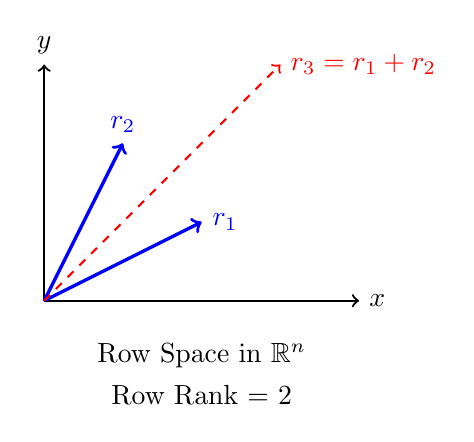
\begin{tikzpicture}
    % Coordinate axes for row space
    \draw[->,thick] (0,0) -- (4,0) node[right]{$x$};
    \draw[->,thick] (0,0) -- (0,3) node[above]{$y$};

    % Row vectors
    \draw[->,very thick,blue] (0,0) -- (2,1) node[right]{$r_1$};
    \draw[->,very thick,blue] (0,0) -- (1,2) node[above]{$r_2$};
    \draw[->,thick,red,dashed] (0,0) -- (3,3) node[right]{$r_3 = r_1 + r_2$};

    % Label for row space
    \node at (2,-0.7) {Row Space in $\mathbb{R}^n$};
    \node at (2,-1.2) {Row Rank = 2};
  \end{tikzpicture}
  \hspace{1cm}
  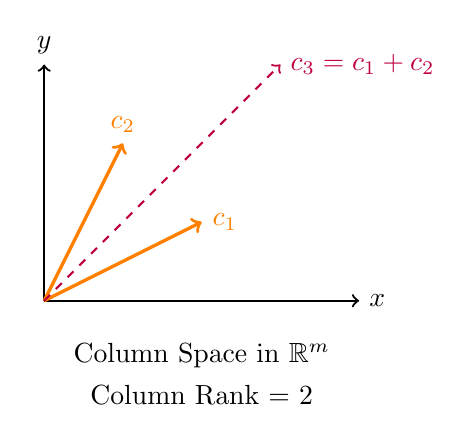
\begin{tikzpicture}
    % Coordinate axes for column space
    \draw[->,thick] (0,0) -- (4,0) node[right]{$x$};
    \draw[->,thick] (0,0) -- (0,3) node[above]{$y$};

    % Column vectors
    \draw[->,very thick,orange] (0,0) -- (2,1) node[right]{$c_1$};
    \draw[->,very thick,orange] (0,0) -- (1,2) node[above]{$c_2$};
    \draw[->,thick,purple,dashed] (0,0) -- (3,3) node[right]{$c_3 = c_1 + c_2$};

    % Label for column space
    \node at (2,-0.7) {Column Space in $\mathbb{R}^m$};
    \node at (2,-1.2) {Column Rank = 2};
  \end{tikzpicture}
\end{center}

Consider a matrix $A = \begin{bmatrix} 1 & 2 & 3 \\ 4 & 5 & 6 \\ 7 & 8 & 9 \end{bmatrix}$:

\begin{itemize}
  \item Rows: $r_1 = [1, 2, 3]$, $r_2 = [4, 5, 6]$, $r_3 = [7, 8, 9]$
  \item Columns: $c_1 = [1, 4, 7]^T$, $c_2 = [2, 5, 8]^T$, $c_3 = [3, 6, 9]^T$
\end{itemize}

We can verify that $r_3 = r_1 + r_2$ and $c_3 = c_1 + c_2$, so both row rank and column rank equal 2.

\begin{center}
  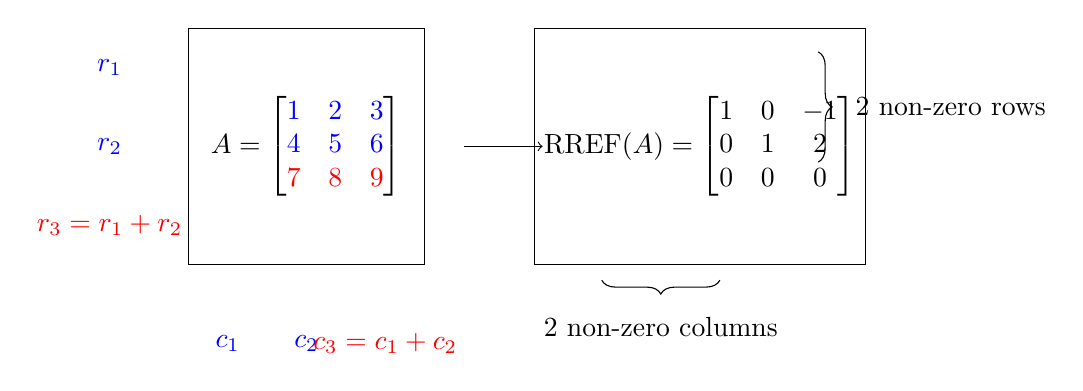
\begin{tikzpicture}
    % Original matrix
    \node[draw, minimum width=3cm, minimum height=3cm] (A) at (0,0) {$A = \begin{bmatrix}
          \textcolor{blue}{1} & \textcolor{blue}{2} & \textcolor{blue}{3} \\
          \textcolor{blue}{4} & \textcolor{blue}{5} & \textcolor{blue}{6} \\
          \textcolor{red}{7}  & \textcolor{red}{8}  & \textcolor{red}{9}
        \end{bmatrix}$};

    % Row and column annotations
    \node[blue] at (-2.5,1) {$r_1$};
    \node[blue] at (-2.5,0) {$r_2$};
    \node[red] at (-2.5,-1) {$r_3 = r_1 + r_2$};

    \node[blue] at (-1,-2.5) {$c_1$};
    \node[blue] at (0,-2.5) {$c_2$};
    \node[red] at (1,-2.5) {$c_3 = c_1 + c_2$};

    % Arrow to RREF
    \draw[->] (2,0) -- (3,0);

    % RREF
    \node[draw, minimum width=3cm, minimum height=3cm] (RREF) at (5,0) {$\text{RREF}(A) = \begin{bmatrix}
          1 & 0 & -1 \\
          0 & 1 & 2  \\
          0 & 0 & 0
        \end{bmatrix}$};

    % Non-zero rows and columns in RREF
    \draw [decorate, decoration={brace, amplitude=5pt}] (6.5,1.2) -- (6.5,-0.2) node[midway, right=10pt] {2 non-zero rows};
    \draw [decorate, decoration={brace, amplitude=5pt, mirror}] (3.75,-1.7) -- (5.25,-1.7) node[midway, below=10pt] {2 non-zero columns};
  \end{tikzpicture}
\end{center}

In the RREF, we see exactly 2 non-zero rows and 2 non-zero columns, confirming rank = 2.

\subsection{Row rank = column rank - Intuitive Explanation}

The key insight is that row operations don't change the relationships between rows or columns, just how they're expressed. Let's visualize why row rank equals column rank:

\begin{center}
  \begin{tikzpicture}
    % Matrix A factorization
    \node at (0,3) {$A = QP$ where $P$ contains a basis for the row space};

    % Matrix A
    \node[draw, minimum width=2cm, minimum height=2.5cm] (A) at (0,0) {$A_{m \times n}$};

    % Matrix Q
    \node[draw, minimum width=1.5cm, minimum height=2.5cm] (Q) at (-3,0) {$Q_{m \times r}$};

    % Matrix P
    \node[draw, minimum width=2cm, minimum height=1.5cm] (P) at (-3,-3) {$P_{r \times n}$};

    % Arrows
    \draw[->] (Q) -- (A) node[midway, above] {$\times P$};
    \draw[->] (P) -- ++(2.5,0) node[right] {Row basis};
    \draw[->] (Q) -- ++(-1.5,0) node[left] {Column combinations};

    \node at (0,-5) {Matrix columns are combinations of $r$ columns from $Q$\\so column rank $c \leq r$};
  \end{tikzpicture}
  \hspace{1cm}
  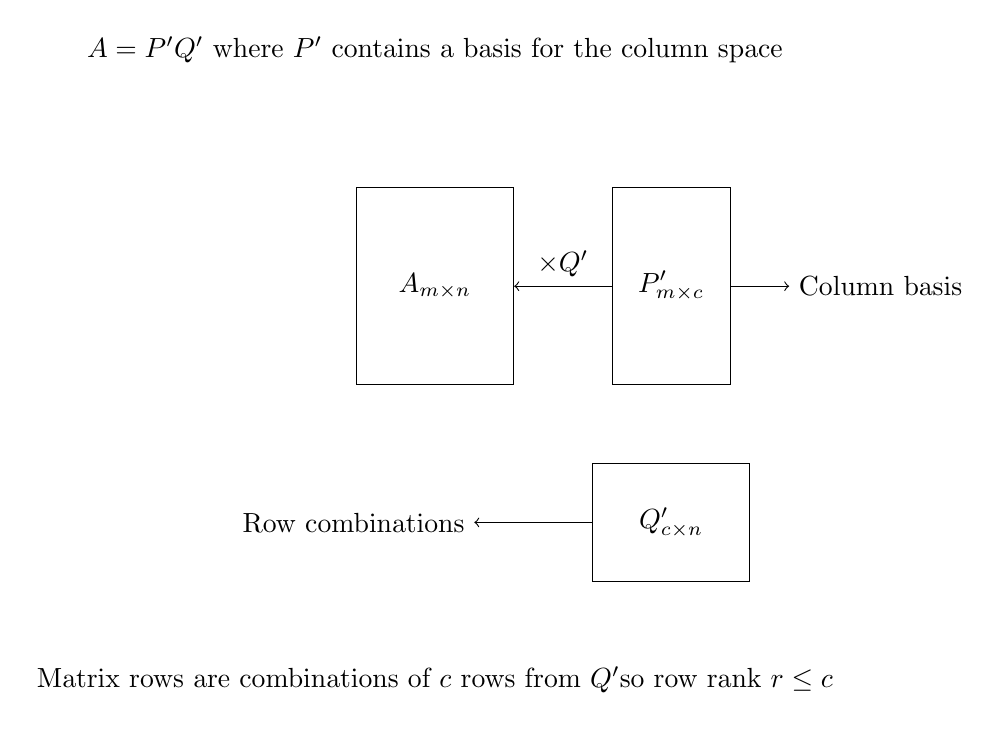
\begin{tikzpicture}
    % Matrix A factorization
    \node at (0,3) {$A = P'Q'$ where $P'$ contains a basis for the column space};

    % Matrix A
    \node[draw, minimum width=2cm, minimum height=2.5cm] (A) at (0,0) {$A_{m \times n}$};

    % Matrix Q prime
    \node[draw, minimum width=2cm, minimum height=1.5cm] (Qp) at (3,-3) {$Q'_{c \times n}$};

    % Matrix P prime
    \node[draw, minimum width=1.5cm, minimum height=2.5cm] (Pp) at (3,0) {$P'_{m \times c}$};

    % Arrows
    \draw[->] (Pp) -- (A) node[midway, above] {$\times Q'$};
    \draw[->] (Qp) -- ++(-2.5,0) node[left] {Row combinations};
    \draw[->] (Pp) -- ++(1.5,0) node[right] {Column basis};

    \node at (0,-5) {Matrix rows are combinations of $c$ rows from $Q'$\\so row rank $r \leq c$};
  \end{tikzpicture}
\end{center}

Since we've shown that $c \leq r$ and $r \leq c$, we must have $c = r$. This allows us to simply talk about the \textbf{rank} of a matrix without specifying row or column.

An intuitive way to understand this equality: imagine the matrix $A$ as a linear transformation. The row rank tells us how much information is contained in the input constraints, while the column rank tells us how many dimensions the output can span. These must be equal because the transformation can't create or destroy dimensions of information.
\end{document}
